\subsection{6.3 样本混合器：稳定的异步混合任务 RL}\label{sample-mixer-stable-asynchronous-mixed-task-rl}

自 MiMo-V2-Flash（Core Team et al., 2026）起，我们一直维护一个 Data
Scheduler，它面向跨数据源的指定训练分布，并配合动态采样器（Yu et al., 2025）与部分
rollout（Kimi Team, 2025）。混合任务 RL 必须在 rollout 时长与过滤率大幅波动的情况下仍保持该分布，
使每个数据源都能得到有效训练。在 25 个已画像的数据源上，平均生成 token 数与活跃 rollout 时长分别相差 90$\times$ 和 66$\times$（图 15），
这要求调度能够适应各数据源的工作负载。为应对这些挑战，我们实现了 Sample Mixer，
用四种机制填充指定训练分布：自适应 rollout 并发设定各数据源的预算，
自适应 rollout 调度在预算内选择数据源，预测式 rollout 派发将新的 rollout 放置到各 rank，样本
回放则覆盖启动与恢复阶段。

自适应 rollout 并发 较慢的数据源需要更多并发
rollout，才能维持相同的训练贡献。对数据源 $i$，设
\(B _ { i }\) 表示每个训练步目标保留的样本组数，\(r _ { i }\) 为估计的组接受率，
\(t _ { i }\) 为估计的活跃 rollout 时长，包含模型
生成与环境交互，但不含训练步之间的暂停。期望生成需求为 $m \_ \{ i \} = \{ B
\_ \{ i \} \} / \{ r \_ \{ i \} \} ; $；在固定训练吞吐下，
所需并发随 \(t _ { i } m _ { i }\) 增长。我们为每个数据源分配
\(( 1 + p _ { i } ) m _ { i }\)
组的调度预算，其中过采样比 \(p _ { i }\) 满足



\begin{figure}[htbp]
\centering
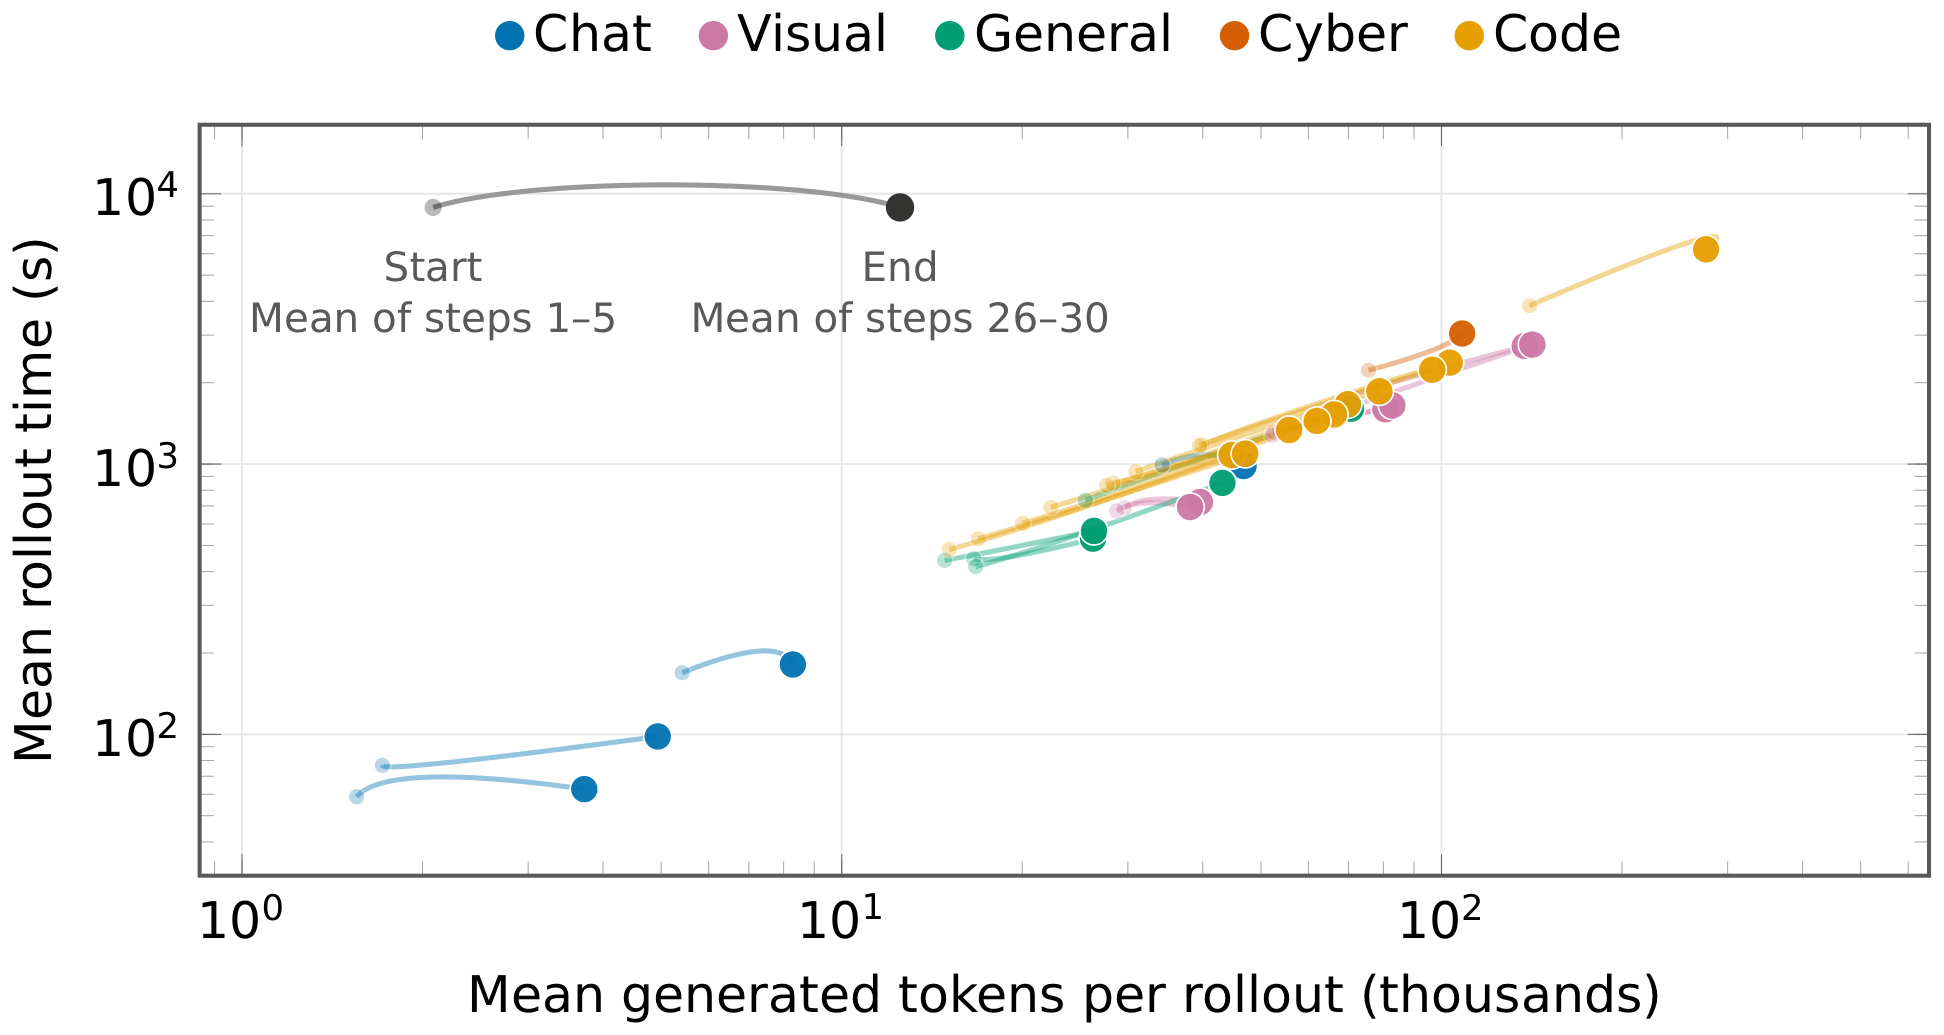
\includegraphics[width=\linewidth]{images_hi/fig15.png}
\caption{25 个数据源上的 rollout 异质性。每条线连接一个数据源的 Start 点（浅色）与其 End 点（实线）；每个点画出该数据源在已完成 rollout 上的平均生成 token 数与平均 rollout 时间（token 在上下文过滤前跨对话上下文求和）。两个坐标轴均为对数尺度。}
\label{fig:15}
\end{figure}


\[
p _ { i } = \mathrm { c l i p } ( c t _ { i } - 1 , p _ { \mathrm { m i n } } , p _ { \mathrm { m a x } } ) , \qquad \frac { \sum _ { i } m _ { i } p _ { i } } { \sum _ { i } m _ { i } } = \bar { p } .\tag{6}
\]

共享因子 $c$ 将 \(p _ { i }\) 的需求加权均值保持在
全局过采样比 \({ \bar { p } } ,\) 处，并受各数据源上界约束。我们随工作负载变化，依据近期计时与接受
统计重新计算该分配。在稳态下，并发
需求随数据源的 rollout 时长与目标增长，随其接受率下降。

自适应 rollout 调度 在这些预算内，调度在长期生成需求
与当前训练批的推进之间取得平衡。若当前批已从数据源 $i$
接受 \(A _ { i }\) 组，则其调度权重为

\[
w _ { i } = \alpha \frac { B _ { i } } { r _ { i } } + ( 1 - \alpha ) \frac { ( B _ { i } - A _ { i } ) ^ { + } } { r _ { i } } ,\tag{7}
\]

其中 \(( x ) ^ { + } = \operatorname* { m a x } ( x , 0 )\)，且
\(\alpha \in [ 0 , 1 ]\)。目标项维持生成需求；
亏空项优先考虑仍有亏空的数据源。这些
权重驱动平滑加权轮询；稳态启动将
\(\alpha = 0 . 5\) 与按 \(t _ { i } m _ { i }\) 比例分配的初始并发结合使用。图 16 的轨迹驱动仿真
在固定并发上限、数据源预算不构成约束的条件下比较了这些策略：在该工作负载下，亏空校正调度 \(( \alpha = 0 . 5 )\)
相比基于亏空的调度
\(\left( \alpha = 0 \right)\) 提升了占用稳定性，相比基于目标的
调度 \(( \alpha = 1 )\) 改善了收集均衡性。仿真时长按图 15 中各数据源
在 End 处的平均 rollout 时间校准。

预测式 rollout 派发 我们联合估计 KV 需求与期望
推理并发，以指导新 rollout 在各 rank 上的准入与放置。按数据源先验估计一个 rollout 的总
序列长度（输入与生成 token），跨上下文求和；
这些先验由已完成的 rollout 更新，并用于估计 KV
需求。仅当一个 rollout 估计 KV 需求的安全余量倍数
能放入目标 rank 剩余的 GPU KV
容量时，我们才准入该 rollout。分层缓存（§6.4）横跨 HBM 与锁页主机内存池：
两层共同保留已准入 rollout 的状态。rollout 时间中用于环境执行的
估计占比将 rollout 并发转换为期望推理并发。我们
用 CUDA graph 捕获所用的最大运行请求数来约束该期望值，从而限制会延长 rollout 生命周期并
增加陈旧度的排队延迟。为在两种约束下最大化吞吐，一个
贪心启发式选择剩余容量最大的可行 rank——即可用并发槽位与剩余 KV
容量（均以序列为单位表示）中的较小者——并在每次放置后更新这两个量。




\begin{figure}[htbp]
\centering
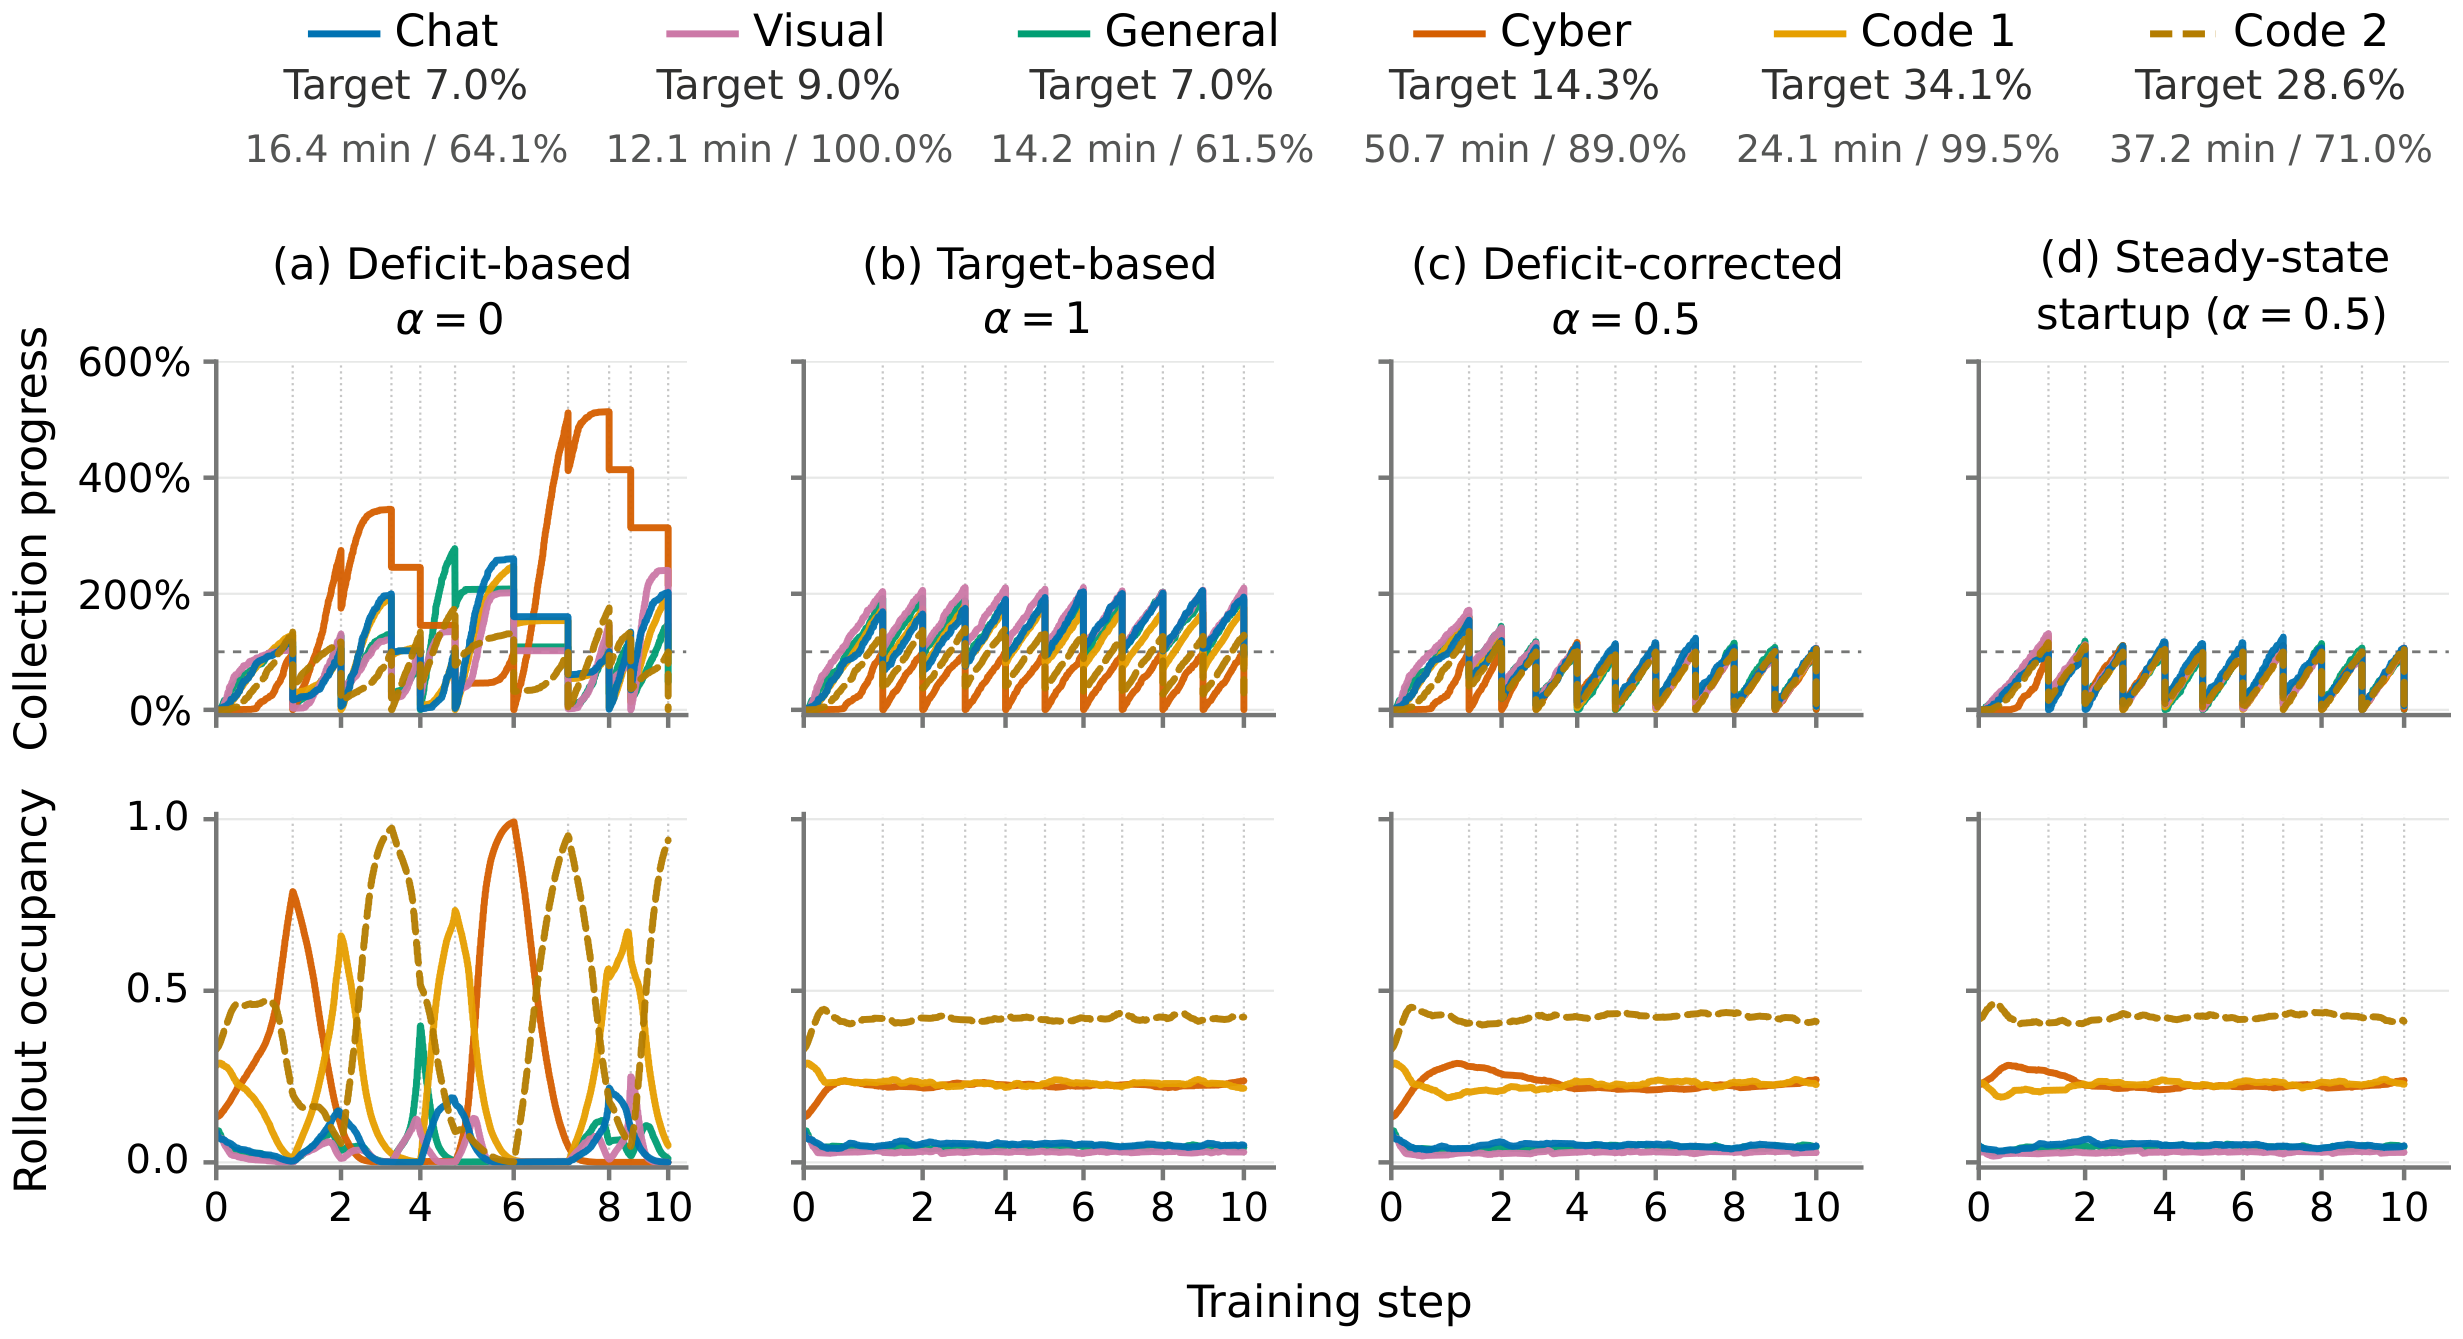
\includegraphics[width=\linewidth]{images_hi/fig16.png}
\caption{六个数据源的轨迹驱动调度仿真。图例：平均时长 / 组接受率。上：收集进度（已接受组数 / 每步名义目标，盈余结转）。下：rollout 占用（已占用序列槽位的份额）。步间距反映经过的时间。虚线标出步边界。训练时间、信用分配延迟、陈旧过期与回放不计入。}
\label{fig:16}
\end{figure}


样本回放 我们使用样本回放来加速从
慢数据源的初始收集。在画像中，启动阶段的样本收集耗时约为持续运行的
1.8$\times$。在慢数据源内部，
较短的 rollout 往往先完成，即使各数据源目标已达成，也会使初始批次
产生偏差。因此，我们在启动或检查点恢复后的第一个收集步中，
复用来自选定慢数据源的已完成 rollout
组，在当前过滤规则下补齐各数据源剩余的亏空。全新启动回放假定
所存 rollout 是在该运行起始策略下生成的；恢复回放则
复用恢复前生成、且仍在各数据源陈旧上限内的已完成 rollout。将回放限制在第一个
收集步，可减少对慢数据源的等待，同时保持
指定的训练分布。



\subsection{6.4 训练/推理一致性与优化}\label{traininginference-consistency-and-optimization}

我们扩展 MiMo-V2-Flash（Core Team et
al., 2026）的 RL 与 OPD 基础设施，仍以 SGLang（Zheng et al., 2024）和 Megatron-LM（Shoeybi
et al., 2019）分别作为推理引擎与训练引擎。在
MiMo-V2.6 中，我们在 rollout 期间使用 MXFP4 作为专家的数据类型。我们
在混合专家（MoE）路由与概率归一化上保持两个引擎
对齐。推理侧，
Context Cache 在跨轮次携带 KV 状态的同时携带路由记录、采样候选集与
视觉输入，并将空闲状态卸载到主机内存。一个在 RL rollout 日志上训练的
草稿模型通过推测解码进一步
加速生成。训练侧，我们降低长序列的内存与通信开销。

训练--推理一致性 为支撑 MiMo-V2.6 系列，我们在每次参数
更新后对专家应用量化--反量化（QDQ）。该量化遵循 rollout 期间
所用 MXFP4 Humming GEMM 内核（vLLM Project, 2026）的数值约束，因此
两个引擎看到完全相同的专家权重。即使参数相同，引擎间的数值差异也可能
改变离散的专家选择；Rollout Routing Replay（R3）（Ma et al., 2025）记录
rollout 期间使用的专家索引，并在训练期间重放它们，
复现所捕获的执行路径。Top-k 与 top-p 采样在受限候选集而非全
词表上重新归一化；我们在 rollout 期间记录每个 token 的候选集（Liu et
al., 2025a; The Microsoft AI Team, 2026），并在其中重新归一化训练的
对数概率，以匹配采样器的归一化。对于
top-p 采样，只有 GPU--CPU 传输是稠密的：我们传输一个固定形状、全词表宽度的位图。
固定形状避免了 GPU--CPU
同步；全宽度则绝不会截断即使跨越
整个词表的候选集。后续所有阶段都是稀疏的：在典型的 top-p
0.97 下，候选集平均不到五个 token。R3 与 top-p
候选集重放的开销都可以忽略，因为负载保持
紧凑，并且不落在关键路径上。

上下文缓存 沿用 MiMo-V2-Flash
（Core Team et al., 2026）的请求级 KVCache，每个对话上下文都有一个持久键：
在同一个策略版本内，后续轮次命中已缓存的 KV——包括
生成的 token——只对新后缀做 prefill。上下文缓存是一个
刻意的有状态选择：缓存状态的生命周期长于每一轮。
因此，专家索引与候选集不会在
中间轮次返回，只在 rollout 最终被收集时返回，
避免了碎片化的逐轮通信与处理。历史
多模态输入既不需要重新哈希，也不需要重新发送：其视觉
token 已经位于缓存的 KV 中。只有新引入的图像
跨进程边界；完整视觉输入仅在
策略更新或缓存未命中后发送。多轮环境交互将
一条轨迹的墙上时钟划分为 GPU 时间（生成）与工具时间
（等待环境）；缓存的层次化扩展
将这种时间划分在空间上体现出来——状态在
GPU 时间驻留于 HBM，在工具时间驻留于锁页主机内存池。卸载与
恢复在旁路 CUDA 流而非计算流上运行，
绝不会阻塞生成。由此，HBM 尽可能用于运行中的请求：
解码批越大，算术
强度与算力利用率越高。

草稿模型加速 RL rollout 默认使用 block-6 DFlash 进行推测
解码，取代从 SFT 继承的多 token 预测（MTP-3）
配置。DFlash 最初在 SFT 策略上训练，
随后在重采样以匹配
RL 训练分布的早期 RL rollout 日志上微调。在该默认配置下，平均
接受长度比 MTP 配置高 31.3\%。在
较大的 RL 批大小下，我们依据端到端
吞吐而非仅凭接受率来选择草稿块大小。更小的草稿块
减少验证工作量：在混合任务 RL 评测中，block-6 相比 block-8 将
全局平均吞吐提升约 6\%，而平均接受长度变化
很小。低精度草稿计算（FP8）
也被用于降低起草开销。在我们的长上下文
工作负载上，经 RL 适配的 FP8 DFlash 相比基线取得约 10.3\% 更高的
单节点吞吐。



训练优化 我们以 1M token 的上下文长度训练 RL。
MiMo-V2.6 将 128-token 滑动窗口层与全
注意力交替堆叠。在上下文并行下，滑动窗口层只交换
其查询能触及的 KV——至多一个窗口大小的
片段——因此每层通信量由窗口而非
序列长度决定。长序列还会抬高内存占用，
MoE 专家不均衡则进一步推高峰值内存。优化器状态保存在
CPU 内存中，仅在参数更新时拷回。所有损失
计算融合进一个内核：策略梯度损失（带或不带 top-p 重新归一化）
与 OPD 损失，可选地连同熵、标签 logit、top-p 概率质量等指标。该融合节省内存
并缩短步时间。
